\documentclass[12pt,spanish,chapterprefix, numbers=noenddot]{book}
\usepackage{amsmath}
\usepackage{amsthm}
\usepackage{fontspec}
\usepackage[a4paper]{geometry}
\geometry{verbose,tmargin=2.5cm,bmargin=2.5cm,lmargin=2.5cm,rmargin=2.5cm,headheight=1cm,headsep=1cm,footskip=1cm}
\setlength{\parskip}{\medskipamount}
\setlength{\parindent}{0pt}
\usepackage{color}
\usepackage{babel}
\addto\shorthandsspanish{\spanishdeactivate{~<>}}

\usepackage{float}
\usepackage{makeidx}
\makeindex
\usepackage{graphicx}
\usepackage{nomencl}
% the following is useful when we have the old nomencl.sty package
\providecommand{\printnomenclature}{\printglossary}
\providecommand{\makenomenclature}{\makeglossary}
\makenomenclature
\usepackage[unicode=true,pdfusetitle,
 bookmarks=true,bookmarksnumbered=false,bookmarksopen=false,
 breaklinks=true,pdfborder={0 0 0},pdfborderstyle={},backref=false,colorlinks=true]
 {hyperref}
\hypersetup{
 allcolors=blue}
\usepackage{listings}
\makeatletter

%%%%%%%%%%%%%%%%%%%%%%%%%%%%%% LyX specific LaTeX commands.
\newcommand{\noun}[1]{\textsc{#1}}
\providecommand\textquotedblplain{%
  \bgroup\addfontfeatures{Mapping=}\char34\egroup}
%% Because html converters don't know tabularnewline
\providecommand{\tabularnewline}{\\}
\floatstyle{ruled}
\newfloat{algorithm}{tbp}{loa}[chapter]
\providecommand{\algorithmname}{Algoritmo}
\floatname{algorithm}{\protect\algorithmname}

%%%%%%%%%%%%%%%%%%%%%%%%%%%%%% Textclass specific LaTeX commands.
\numberwithin{equation}{section}
\numberwithin{figure}{section}
\providecommand*{\code}[1]{\texttt{#1}}

%%%%%%%%%%%%%%%%%%%%%%%%%%%%%% User specified LaTeX commands.
%Para que las URLs de la bibliografía se pueda pinchar
\usepackage{url}

%Cabeceras y pies de página
\usepackage{fancyhdr}
\pagestyle{fancy}
\lhead[\rightmark]{}
\rhead[]{\leftmark}
\cfoot{\thepage}

%Para que los índices respeten los espacios de las nuemraciones
\usepackage[tocindentauto]{tocstyle}
\usetocstyle{standard}

%Para que ponga "Índice de Tablas" en vez de "Indice de Cuadros"
\addto\captionsspanish{
\def\tablename{Tabla}
\def\listtablename{\'Indice de tablas}
}

%Para que las páginas en blanco no tengan cabecera ni número de página
\makeatletter
\renewcommand*{\cleardoublepage}{\clearpage\if@twoside \ifodd\c@page\else
\hbox{}%
\thispagestyle{empty}%
\newpage%
\if@twocolumn\hbox{}\newpage\fi\fi\fi}
\makeatother



\usepackage{chngcntr}
\counterwithout{figure}{chapter}
\counterwithout{figure}{section}
\counterwithout{table}{chapter}
\counterwithout{algorithm}{chapter}

\setcounter{tocdepth}{3}

\AtBeginDocument{
  \def\labelitemii{\(\circ\)}
  \def\labelitemiii{\(\triangleright\)}
}

\makeatother

\usepackage{listings}
\lstset{basicstyle={\ttfamily},
breaklines=true}
\usepackage[style=numeric,backref=true]{biblatex}
\def\eqdeclaration#1{, véase la ecuación\nobreakspace(#1)}
\def\pagedeclaration#1{, página\nobreakspace#1}
\def\nomname{Nomenclatura}
\renewcommand{\lstlistingname}{Listado de código}

\addbibresource{./refs.bib}
\begin{document}
\frontmatter

\begin{titlepage}

\begin{center}

\includegraphics[width=8cm]{Figs/logoURJC}
\par\end{center}

\begin{center}
Escuela Técnica Superior de Ingeniería de Telecomunicación
\par\end{center}

\vspace{4cm}

\begin{center}
{\LARGE{}MOVIMIENTO DE UN BRAZO ROBÓTICO EN EL ENTORNO EDUCATIVO UNIBOTICS}{\LARGE\par}
\par\end{center}

\vspace{4cm}

\begin{center}
{\large{}Memoria del Trabajo Fin de Grado}{\large\par}
\par\end{center}

\begin{center}
{\large{}en Ingeniería en Sistemas Audiovisuales y Multimedia}{\large\par}
\par\end{center}

\vspace{4cm}

\begin{center}
{\large{}Autor: Ignacio Malo Segura}{\large\par}
\par\end{center}

\begin{center}
{\large{}Tutor: José María Cañas Plaza}{\large\par}
\par\end{center}

\begin{center}
{\large{}Co-tutor: José Francisco Vélez Serrano}{\large\par}
\par\end{center}

\begin{center}
2019
\par\end{center}

\end{titlepage}

\chapter*{Agradecimientos}

\chapter*{Resumen}

\tableofcontents{}

\mainmatter

\chapter{Introducción}

\section{El sector: presente y futuro}
El mercado de la robótica está llamado a convertirse en uno de los más importantes del presente siglo, alcanzando una valoración estimada superior a los 28 billones de euros en el año 2018. En los últimos años ha experimentado un gran crecimiento y se espera que continúe en los próximos años, con una previsión de un 25\% de revalorización para los próximos 5 años. 
La explicación más obvia para este hecho se fundamenta en la aún reciente tendencia a la automatización de tareas a nivel empresarial, sumado a un incremento en la compra de tecnología robótica a nivel usuario.
Ahora bien, ¿cuáles son las razones que explican este crecimiento de la automatización, y hacia dónde nos lleva?. Aunque hay algunas características propias del ser humano(creatividad, impredecibilidad, lgunas de las razones que explican las tendencias comentadas son:
\begin{itemize}
\item Aumento de la eficiencia 
\item Productividad sin descanso
\item Reducción de costes
\item Evita el error humano
\item Más precisión
\item Control de errores
\end{itemize}
Por otro lado, uno de los factores clave para comprender el futuro del sector es el impacto que puede tener en el mercado laboral tal y como lo conocemos actualmente. Algunos estudios apuntan que dentro de 35 años, alrededor del 60\% de los trabajos estarán automatizados, con el impacto que eso conlleva para los diferentes trabajadores, que podrían perder puestos de trabajo en favor de profesionales del software que serán necesarios para afrontar el proceso de transición, y posterior mantenimiento de esta digitalización. 

Los perfiles STEM(carreras relacionadas con ciencia, tecnología, ingeniería y matemáticas) van a ser cada vez más demandados en los próximos años, con el hándicap de que los nuevos profesionales relacionados con estas áreas disminuyen cada año. 
Si vemos los datos de empleos relacionados con alta tecnología en nuestro país, y los comparamos con el resto de países europeos, observamos que el porcentaje de empleos de este tipo es muy pobre en la gran mayoría de regiones españolas, a excepción de Madrid y, en menor medida, la zona noreste de la península. 


\section{}
\subsection{}
\subsection{}

\chapter{Objetivos}
\section{}

\chapter{Infraestructura}
En este capítulo se detalla el software necesario para el desarrollo de las aplicaciones construidas. Desde ROS Kinetic y JdeRobot como middlewares robóticos, pasando por la herramienta MoveIt! para facilitar el trabajo con robots(PR2) hasta el simulador Gazebo. Todo ello corriendo en el sistema operativo Ubuntu 16.04 y desarrollado en Python y C++.  Las comunicaciones entre los distintos componentes utilizan el motor de comunicaciones ICE además de ROS topics. 
\section{PR2}
El robot sobre el que se han desarrollado las aplicaciones es el PR2 de Willow Garage, empresa especializada en robótica responsable también del software ROS y otras herramientas open-source. Se compone de dos brazos(derecho e izquierdo)capaces de generar un amplio abanico de oportunidades de movimiento que no serían posibles con un único brazo, y que terminan en una pinza o 'gripper' que permite agarrar objetos. El nombre viene de Personal Robot 2, haciendo referencia a la idea de que fuera un asistente en casa y no un robot industrial como la mayoría de los comercializados hasta el momento.
Su diseño modular permite integrarlo con otros grippers, brazos o sensores.
\begin{center}
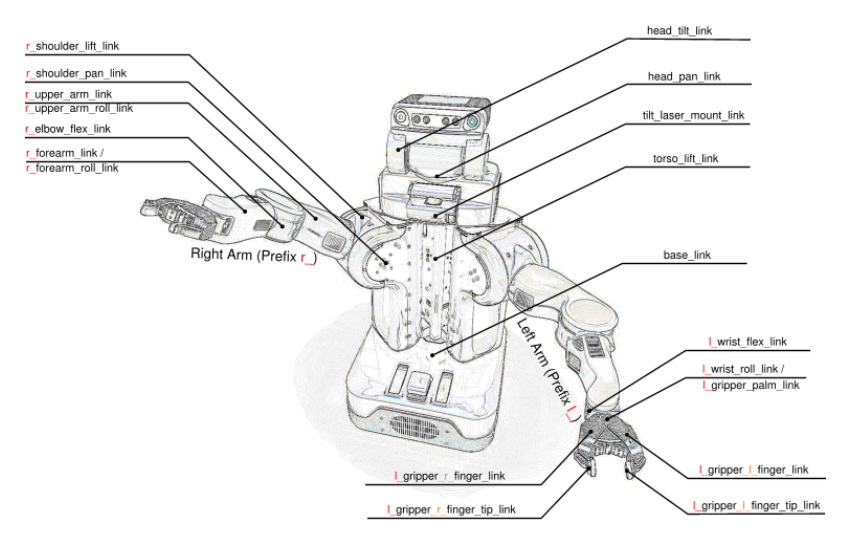
\includegraphics[width=12cm]{Figs/PR2_structure.png}
\end{center}
Su muñeca tiene dos grados de movimiento, que se suman a la libertad que aportan las articulaciones del hombro y el codo para permitir prácticamente cualquier movimiento necesario para una labor doméstica.
Además de su estructura, una característica fundamental del robot PR2 son las cámaras y láseres que permiten conocer el entorno y actuar según lo que percibe: detectar objetos, saber a qué distancia se encuentran e identificar zonas objetivo permiten llevar a cabo acciones como abrir una puerta o llevar objetos de un lugar a otro.
\subsection{Microsoft Kinect}
La cámara Kinect permite conocer el entorno a través de imágenes procesadas en tiempo real. 
Contiene un sensor de color(RGB) y uno de profundidad, y se sitúa en la parte superior del robot. 

\begin{center}
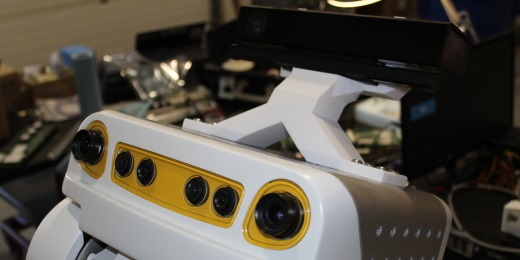
\includegraphics[width=12cm]{Figs/kinect.jpg}
\end{center}


\section{Gazebo}
Este simulador open source nació en el año 2002 en la Universidad del Sur de California(USC) como proyecto entre un profesor y uno de sus estudiantes. El objetivo era poder trabajar con robots bajo condiciones de alta fidelidad, pensando principalmente en entornos exteriores. Se comenzó a integrar con ROS en 2009 y dos años después la citada Willow Garage comenzó a financiar el desarrollo para este software, del que se hizo cargo la Open Source Robotics Foundation(OSRF).
Gazebo fue adaptado para participar en la prestigiosa DARPA Robotics Challenge (DRC) en el año 2013. Hay una comunidad activa detrás del proyecto que permite introducir mejoras, resolver bugs y consultar dudas técnicas.

Como simulador de robótica, lo que ofrece es crear aplicaciones para robots sin necesidad de depender de la máquina física. Así, las aplicaciones creadas para un modelo concreto podrán utilizarse posteriormente en el mundo real sin necesidad de realizar modificaciones, disminuyendo tanto los costes tanto económicos como derivados de la peligrosidad de las pruebas en fase de desarrollo.
Ofrece visualización 3D y un potente motor de físicas para, en el caso de un brazo robótico, poder determinar parámetros como fricción, rango de movimiento, colisiones etc.
\begin{center}
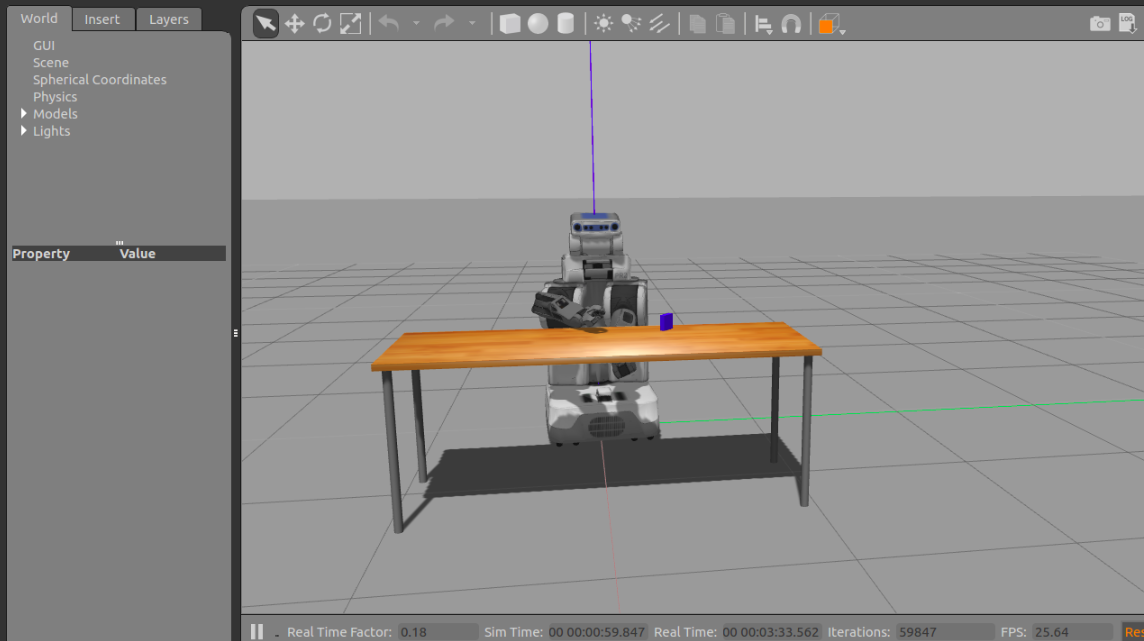
\includegraphics[width=12cm]{Figs/GazeboWorld_PR2.png}
\end{center}
La simulación nace a partir de un fichero launch que arranca Gazebo. El entorno de la simulación está compuesto por un world que contiene diferentes models. Estos modelos están definidos en un fichero con formato SDF con los siguientes componentes principales:
\begin{itemize}
\item Links: contiene las propiedades físicas de un trozo del modelo, incluyendo algunas de visualización y colisión, sensores, inercias o iluminación.
\item Joints: conexión entre dos links.
\item Plugins: librería externa que controla un modelo. 
\end{itemize}
La versión utilizada para este proyecto es Gazebo7.

\section{JdeRobot}
Este software open source permite desarrollar aplicaciones en el campo de la Robótica a partir de código C++, Python o JavaScript. La compatibilidad con ROS, principalmente con la versión Kinetic es una de las grandes ventajas de esta herramienta.  Los diferentes nodos o componentes se comunican a través del framework ICE(Internet Communications Engine) o de mensajes ROS. Ambas opciones permiten realizar dichas comunicaciones de forma agnóstica al lenguaje en el que están desarrollados los componentes.  
De esta estructura parte JdeRobot-Academy, una iniciativa para el aprendizaje en Robótica y Visión Computacional que incluye múltiples ejercicios para que los estudiantes puedan entender y añadir su propio código. JdeRobot  contiene una amplia variedad de componentes y librerías que pueden ser reutilizados por la comunidad de desarrolladores. 
La última versión estable es la 5.6.4, lanzada en mayo de 2018. Uno de los últimos hitos es su participación en el Google Summer of Code 2018. 

\section{ROS Kinetic}
Framework para el desarrollo de software para robots. Nació en 2007 en el Laboratorio de Inteligencia Artificial de Standford. La arquitectura de ROS(Robot Operating System) se basa en nodos que se comunican a través de mensajes, lo que nos permite obtener grafos fácilmente.
Es un sistema de código abierto que encarga de mantener la OSRF(Open Source Robotics Foundation). Aporta al usuario herramientas como por ejemplo planificación de movimiento(MoveIt) o reconocimiento del entorno y visualización (Rviz), además de soporte para un amplio abanico de Robots. 
La versión Kinetic fue lanzada en mayo de 2016, enfocada al uso desde Ubuntu 16.04. La versión Gazebo7 es la recomendada en ROS Kinetic para este simulador. 
-Estructura y comunicaciones
Un paquete de ROS agrupa varios programas o nodos con funcionalidades similares. Estos nodos se comunican  a través de mensajes, llamados ROS Topics, que les permiten interactuar entre sí. 
ROS Core es la herramienta encargada de arrancar el nodo máster y gestionar todas las comunicaciones, por lo que es la primera que debe ser arrancada. Es lanzado automáticamente con los ficheros .launch, que serán muy habituales en el desarrollo. 
\begin{lstlisting}
~$ roscore
\end{lstlisting}
Para ejecutar un nodo, necesitaremos el paquete y el nombre del nodo: 
\begin{lstlisting}
~$ rosrun turtlesim turtlesim_node
\end{lstlisting}

Una vez lanzado el nodo, podemos publicar topics de un tipo concreto que el nodo comprenda, consiguiendo así que realice una acción determinada. Estas comunicaciones son la base del desarrollo con robots en ROS. 
\begin{lstlisting}
~$ rostopic pub -1 /turtle1/cmd_vel geometry_msgs/Twist -- '[2.0, 0.0, 0.0]' '[0.0, 0.0, 1.8]'
\end{lstlisting}

También se pueden obtener por línea de comandos los mensajes publicados en un topic determinado.
\begin{lstlisting}
~$ rostopic echo /turtle1/cmd\_vel
\end{lstlisting}

ROS dispone de herramientas como rqt que permiten observar grafos de las comunicaciones actuales. Si seguimos con el ejemplo de turtlesim:
\begin{center}
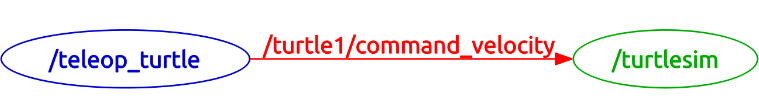
\includegraphics[width=12cm]{Figs/teleopTurtle.png}
\end{center}
\begin{lstlisting}
$ rosrun rqt_graph rqt_graph
\end{lstlisting}
Podemos ver en cualquier momento los nodos o topics disponibles con los siguientes comandos: 
\begin{lstlisting}
~$ rosnode list 
~$ rostopic list
\end{lstlisting}

\section{ICE}
Se trata de un framework RPC(Remote Procedure Call) compatible con lenguajes como C++, C\#, Java, JavaScript o Python. Nace a partir de un modelo cliente-servidor con el objetivo de permitir la comunicación entre distintos lenguajes y sistemas operativos. Esta abstracción ofrece al desarrollador la capacidad de despreocuparse por cómo se gestionan las comunicaciones entre los diferentes módulos para así enfocarse en el problema a resolver. Permite comunicaciones bidireccionales, tanto síncronas como asíncronas. 

Fue diseñado para aplicaciones que requieren un performance y escalabilidad exigentes, minimizando el consumo de CPU y ancho de banda. IceSSL permite añadir seguridad a las comunicaciones, a través de autenticación y encriptación de los datos que viajan en las llamadas. 

\section{C++}
Este lenguaje de programación fue creado por Bjarne Stroustrup en 1979, que lo bautizó en sus inicios como ‘C con clases’. No en vano tiene una sintaxis similar a la de C, manteniendo el vínculo con el lenguaje del que proviene y añadiendo mecanismos de programación orientada a objetos a su predecesor. Su nombre además hace referencia a ese C incrementado, mejorado. 
Es un lenguaje fuertemente tipado, combinado y portátil. Se rige por un estándar de ISO(International Organization for Standardization) cuya última versión es C++17, lanzada ese mismo año. 

El hecho de ser un lenguaje con un grado de complejidad elevado supone una gran versatilidad y potencia, pero también una curva de aprendizaje elevada para dominarlo.
Algunos IDEs recomendados para trabajar con C++ son VisualStudio y Code:: Blocks. 
Como curiosidad, se trata del tercer lenguaje de programación más popular en 2018 según el conocido ranking de TIOBE, sólo por detrás de Java y C. Alcanzó su máximo de popularidad 2003 según los datos de esta empresa de software. (https://www.tiobe.com/tiobe-index/)

\section{Python}
Fue creado en los años 80 por Guido van Rossum. Es un lenguaje de programación interpretado, que utiliza tipado dinámico. Su sintaxis está enfocada a ser fácilmente legible, lo que hace que tenga una curva de aprendizaje suave en relación con otros lenguajes como Java o el propio C. Soporta programación orientada a objetos y es multiplataforma.

Una característica interesante es que puede extenderse con módulos de C o C++.
Según el mencionado ranking TIOBE, Python es el cuarto lenguaje de programación en popularidad llegando al máximo nivel en 2011. 

Se ha utilizado la versión 2.7.12 debido principalmente a su compatibilidad con ROS Kinetic. En este lenguaje se han desarrollado las aplicaciones de planificación de movimientos y pick\&place. 

\subsection{OpenCV}
Librería de código abierto enfocada a proyectos de visión artificial, con interfaces disponibles para varios lenguajes de programación(C++, Python, Java). 
Open Source Computer Vision Library es muy utlizada, con un número de descargas de alrededor de 15 millones y una comunidad de 47000 seguidores.  
Su integración en el proyecto permite aprovechar, en un entorno robótico, toda la potencia del análisis de imágenes. 

\section{MoveIt!: Motion Planning Framework}
MoveIt! nació en octubre del año 2011 con la idea de agrupar todos los avances relacionados con planificación de movimientos, manipulación, percepción 3D, cinemática, control y navegación en una única herramienta. Actualmente es el software open-source más utilizado para manipulación con robots, con más de 65 autómatas soportados. 
Tiene un nodo principal llamado move\_group que actúa como integrador, permitiendo a todos los componentes comunicarse entre sí realizando las acciones soportadas. 
Se puede acceder a move\_group por tres vías: C++, Python y RVIZ.
\begin{center}
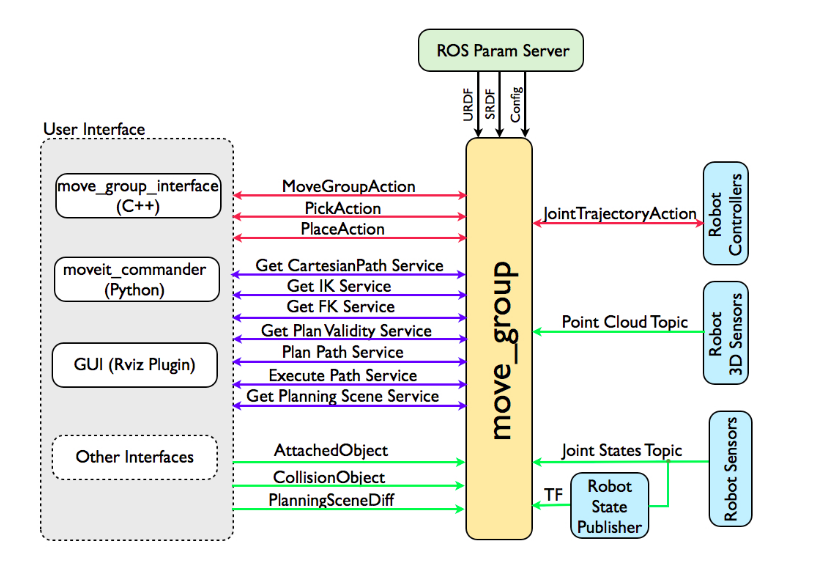
\includegraphics[width=12cm]{Figs/moveGroup.png}
\end{center}
Como se puede ver en el esquema, move\_group necesita varios parámetros de entrada:
\begin{itemize}
\item URDF(Universal Robot Description Format): Es el formato que utiliza ROS para la descripción del robot. Se ha utilizado el del paquete ‘pr2\_description’, correspondiente al autómata utilizado.
\item SRDF(Semantic Robot Description Format) complementa al URDF, añadiendo más información como grupos de joints, configuraciones por defecto para el robot o chequeo de colisiones. Para construir este fichero, se recomienda utilizar el MoveIt! Setup Assistant. Esta herramienta permite configurar cualquier robot para ser utilizado en MoveIt! A través de una interfaz gráfica que simplifica el trabajo. 
\item MoveIt! Configuration: Incluye otros ficheros de configuración específicos de MoveIt!, normalmente generados también a través del Setup Assistant. Contienen información necesaria para planificación de movimientos, cinemática o percepción del entorno.
\end{itemize}
Las principales interfaces de MoveIt! Permiten acceder a las diferentes funcionalidades a través de código C++. Sin embargo, existe un paquete llamado moveit\_python que permite acceder a las principales interfaces de MoveIt! utilizando python:
\begin{itemize}
\item MoveGroupInterface: Utilizada para acceder a move\_group y mover el brazo. 
\item PlanningSceneInterface: Utilizada para añadir o eliminar objetos al entorno y cambiar su apariencia, ya sean conectados o de colisión. 
\item PickPlaceInterface: Utilizada para realizar acciones de pick\&place.
\end{itemize}

Con el objetivo de conseguir la integración de MoveIt! con Gazebo, y poder así enviar los movimientos al robot real(o simulado), debemos configurar correctamente los controladores. Para ello necesitaremos dos ficheros clave: controllers.yaml y joint\_names.yaml.  En ellos se especifican el tipo de mensajes que el robot recibe y las joints que controla.  

\chapter{Aplicación con brazo robótico y planificación de trayectorias}
En este capítulo se describirán en detalle tanto el objetivo como el desarrollo técnico de la práctica "Movimiento de un brazo robótico" para el entorno Unibotics. 
Incluye el enunciado de la misma, la infraestructura necesaria y la plantilla de código python a utilizar. 

\section{Enunciado}

En este capítulo abordaremos el desarrollo de la solución escogida como objetivo del proyecto. Incluye la planificación de trayectorias con obstáculos en un entorno simulado, el reconocimiento de objetos analizando espacios de color, y la planificación y ejecución de movimientos. 

\begin{figure}[hbt!]
\centering
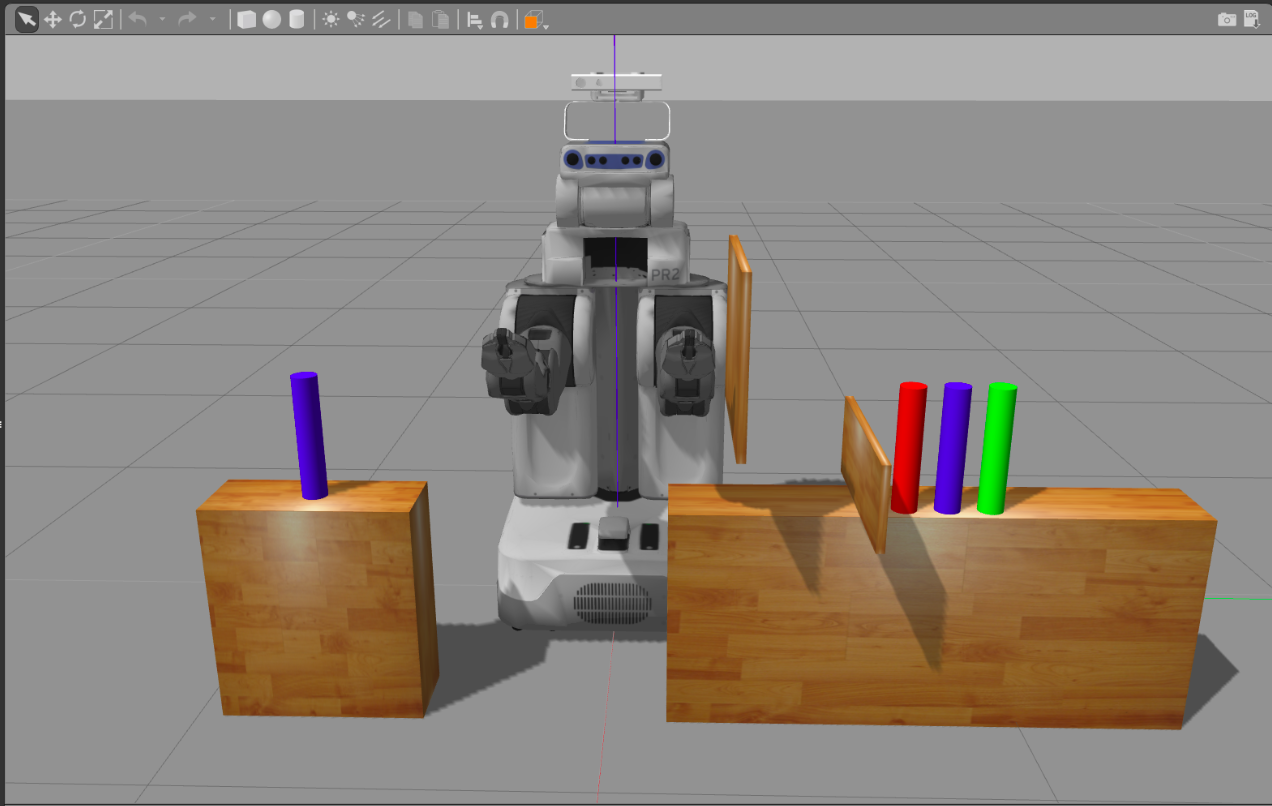
\includegraphics[width=12cm]{Figs/tfg_gazebo_world.png}
\par
\caption{\label{fig:Mundo-gazebo}Mundo Gazebo que incluye todo lo necesario para el desarrollo de la práctica: zonas,objetos,robot y obstáculos.}
\end{figure}

El escenario de la práctica consiste en un mundo Gazebo(Fig. \ref{fig:Mundo-gazebo}) que incluye dos zonas de acción(A y B) y un total de cuatro objetos, uno en la primera zona y tres en la segunda. Entre ellas, un robot PR2 y algunos obstáculos. Los objetos en la zona B tendrán los colores rojo, verde y azul, y el de la zona A tiene únicamente uno de los colores mencionados(azul por defecto). Una vez presentado el mundo, a continuación se relatará a grandes rasgos cuál es el funcionamiento esperado para la práctica. 

En primer lugar,  el robot PR2 moverá la cabeza y observará la Zona A. En ese momento, debe ser capaz de obtener las imágenes de la cámara Kinect que incorpora, que serán analizadas mediante código python para determinar si hay o no un objeto y de qué color es. 
Después, conociendo el color objetivo y las posiciones de los objetos en la zona B, será capaz de planificar ,y posteriormente ejecutar, una trayectoria que le sitúe frente al objeto en la zona B cuyo color coincida con el observado en la zona A. Para ello será necesario gestionar la planificación de trayectorias evitando los obstáculos necesarios y, por último, realizar un movimiento de derribo.




\section{Infraestructura}
Esta sección tiene como objetivo mostrar los elementos necesarios para lograr una práctica completa de planificación. Entre ellos se incluyen el mundo creado en Gazebo y todo lo que ello contiene, como el robot PR2 y los plugins utilizados para el procesado de imagen.  

\subsection{Mundo Gazebo}
En primer lugar, ha sido necesaria la creación de un mundo en Gazebo que contiene los objetos a detectar y empujar, las dos zonas de acción, los obstáculos, el robot PR2 y la cámara Kinect.
La cámara Kinect se incorpora en la parte superior de la cabeza del robot, de forma que se encuentran completamente integrados y podemos controlar la visión del robot a través de movimientos en su parte superior.
Para lanzar este entorno, se debe ejecutar un fichero .launch [\ref{alg:tfg-launch}], que pondrá en funcionamiento los modelos necesarios para las dos zonas de referencia, los modelos de los objetos y obstáculos, y el robot PR2 con todos sus controladores. La cámara Kinect integrada se pasa como parámetro, y está configurada para aparecer por defecto. 
\vspace{20pt}
\begin{algorithm}[htb!]
\begin{lstlisting}[breaklines=true,language=python]
<launch>
  <!-- start up world -->
  <arg name="gui" default="true"/>
  <arg name="headless" default="false" />
  <arg name="debug" default="false" />
  <arg name="paused" default="true"/>
  <arg name="KINECT2" default="$(optenv KINECT2 true)" />
  <include file="$(find gazebo_ros)/launch/empty_world.launch">
    <arg name="world_name" value="worlds/tfg_world.world"/> 
    <arg name="gui" value="$(arg gui)" />
    <arg name="headless" value="$(arg headless)" />
    <arg name="paused" value="$(arg paused)" />
    <arg name="debug" value="$(arg debug)" />
    <arg name="use_sim_time" value="true" />
  </include>
  <!-- start pr2 robot with Kinect camera -->
  <include file="$(find pr2_gazebo)/launch/pr2.launch">
    <arg name="KINECT2" value="$(arg KINECT2)" />
  </include>
</launch>
\end{lstlisting}

\caption{\label{alg:tfg-launch}Fichero .launch para el mundo gazebo y el robot PR2.}
\end{algorithm}

\subsubsection{Modelo PR2}
El modelado principal del robot PR2 utilizado en esta práctica corresponde a los paquetes pr2\_gazebo y pr2\_common. Se trata de paquetes disponibles para ROS Kinetic, que contienen todo lo necesario para simular el robot de Willow Garage en Gazebo, como  información sobre joints, físicas, colisiones o dimensiones.
De cara a lograr el objetivo final, ha sido necesario hacer ligeras modificaciones para añadir una cámara Kinect \cite{gazebo_plugins} en la parte alta del modelo, así como desactivar el sensor láser que utiliza por defecto, para evitar generar ruido en las imágenes RGB obtenidas. 

\subsubsection{Modelos adicionales}
Se ha desarrollado un fichero .world que define los modelos necesarios para la consecución de la práctica. Para cada uno de los elementos se establecen su posición, como será su visualización, sus criterios de colisión y sus dinámicas. 
Para ello se utiliza el formato SDF \cite{sdf_format}, open-source y basado en XML y que permite describir modelos de cualquier complejidad a través de sencillas etiquetas, desde esferas o prismas, hasta robots completos.

\vspace{20pt}
	\begin{lstlisting}[frame=single]
  <model name="base_A">
   <pose>0.6 -0.7 0.275 0 0 0</pose>
   <static>true</static>
   <link name="link">
    <collision name="surface">
     <pose>0.0 0.0 0.0 0 0 0</pose>
     <geometry>
      <box>
       <size>0.2 0.5 0.55</size>
      </box>
     </geometry>
     <surface>
      <friction>
       <ode>
        <mu>10</mu>
        <mu2>10</mu2>
       </ode>
      </friction>
     </surface>
    </collision>
    <visual name="visual1">
     <pose>0.0 0.0 0.0 0 0 0</pose>
     <geometry>
      <box>
       <size>0.2 0.5 0.55</size>
      </box>
     </geometry>
     <material>
      <script>
       <uri>file://media/materials/scripts/gazebo.material</uri>
       <name>Gazebo/Wood</name>
      </script>
     </material>
    </visual>
   </link>
  </model>
	\end{lstlisting}

\section{Plantilla}
Como se muestra en la sección anterior, el nodo python será capaz de detectar a partir de una imagen de entrada si hay algo azul, rojo o verde delante de la cámara, y en caso afirmativo, determinar si es el objeto esperado, eliminando posibles errores provocados por ruido. 
Para ello, el nodo importa las librerías cv2 y rospy. Además, para la planificación de trayectorias, se importan moveit\_commander y los distintos mensajes de MoveIt necesarios para la planificación de trayectorias.

Existen dos ficheros python, uno llamado final\_prototype\_template\_ready.py y otro llamado template.py[\ref{alg:template-py}]. 
El primero contiene la mayor parte de la complejidad de la práctica, y tiene como objetivo abstraer al usuario final de los entresijos necesarios para hacer funcionar un brazo robótico con MoveIt! y gestionar imágenes con OpenCV, simplificando dichas tareas a través de algunas funciones sencillas. 
De esta manera, el alumno tendrá disponibles las siguientes interfaces desde el fichero template.py: 

\begin{itemize}
\item look\_at\_object(x,y,z): Mueve la cabeza del robot PR2 configurando y enviando un mensaje PointHeadGoal con los parámetros recibidos.
\item Subscriber: es el encargado de llamar al callback para que realice acciones cuando se recibe una imagen en el topic.
\item convert\_to\_cv2(msg): convierte el mensaje recibido en el callback en una imagen preparada para trabajar con OpenCV.
\item convert\_to\_hsv(img): convierte una imagen BGR al espacio de color HSV. 
\item save\_image(img): guarda la imagen en formato .jpeg en un directorio local. 
\item def detect\_objects(img, lower, upper, color): recibe como parámetros los valores mínimos y máximos de HSV y aplica la máscara para detectar objetos de color teniendo en cuenta su tamaño y eliminando falsos positivos. 
\item start\_planning(): instancia los objetos necesarios para obtener y modificar valores del robot, la escena y la planificación. Añade los objetos a considerar como obstáculos en la planificación y configura tanto el tiempo máximo como el número de intentos para la misma. 
\item set\_orientation\_constraints(link, orientation, x\_tol,y\_tol,z\_tol): define restricciones de tolerancia para cada eje de una determinada articulación del robot. 
\item move\_to\_goal(color): planifica y ejecuta un movimiento al objeto destino del color pasado como parámetro. 
\end{itemize}

\vspace{20pt}
\begin{algorithm}[htb!]
	\begin{lstlisting}[breaklines=true,language=python]    
def image_callback(msg):
 global count
 count=count+1
 if count==1:
  cv2_img = convert_to_cv2(msg)
  save_image(cv2_img)
  hsv_img = convert_to_hsv(cv2_img)
  save_image(hsv_img)
  lower_red= np.array([H_min_R,S_min,V_min])
  upper_red= np.array([H_max_R,S_max,V_max])
  lower_blue = np.array([H_min_B,S_min,V_min])
  upper_blue = np.array([H_max_B,S_max,V_max])
  lower_green = np.array([H_min_G,S_min,V_min])
  upper_green = np.array([H_max_G,S_max,V_max])
  objects_detected={"red":0,"green":0,"blue":0}
  detected_color=detect_objects(cv2_img,low_red,up_red,"red")
  objects_detected["red"]=detected_color
  detected_color=detect_objects(cv2_img,low_green,up_green,"green")
  objects_detected["green"]=detected_color
  detected_color=detect_objects(cv2_img,low_blue,up_blue,"blue")
  objects_detected["blue"]=detected_color
  start_planning()
  set_orientation_constraints("l_wrist_roll_link",1.0,0.5,0.5,0.5)
  for x in objects_detected:
   if objects_detected[x]==1:
    move_to_goal(x)
  rospy.spin()
def main():
 rospy.init_node('image_listener')
 x = 0.7
 y = -0.7
 z = 0.4
 look_at_object(x,y,z)
 count=0
 image_topic = "/head_mount_kinect2/rgb/image_raw"
 rospy.Subscriber(image_topic, Image, image_callback)
 rospy.spin()
	\end{lstlisting}
\caption{\label{alg:template-py}Plantilla simplificada para la práctica de planificación de trayectorias}
\end{algorithm}

\chapter{Solución de referencia}
\section{Procesamiento de imagen}
Para generar una posición de destino correcta, es necesario analizar la imagen proporcionada por la cámara adherida al robot  e identificar el objeto en la zona de inicio, si es que lo hay. 
A continuación profundizaremos en los elementos que hacen posible este proceso y como se implementa cada uno de ellos en nuestra práctica de planificación de trayectorias. 

\subsection{Cámara Kinect y ROS topic} 
La cámara Kinect se incorpora en la cabeza del robot, y utiliza el plugin openni\_Kinect [\ref{alg:kinect2-xacro}]. Éste permite obtener imágenes con resolución 680x480 y formato BGR, con 8 bits para cada uno de los colores primarios de la luz y por tanto un total de 24 bits por píxel. Además, al tratarse de una de las comúnmente llamadas cámara RGB-D, ofrece imágenes de profundidad que permitirían detectar lo cerca o lejos que se encuentra un objeto de la cámara. El plugin está configurado para refrescar las imágenes cada segundo, de forma que se puedan detectar de forma dinámica cambios en el entorno.
En nuestro caso, necesitaremos controlar esto para recibir una única imagen y que ello suceda cuando el robot se encuentre mirando a la zona destino, de forma que no se tengan problemas innecesarios de procesamiento debido a código ineficiente.

\vspace{20pt}
\begin{algorithm}[h!]
	\begin{lstlisting}[breaklines=true,language=python]    
<xacro:macro name="kinect2_rgb_gazebo_v0" params="link_name frame_name camera_name">
  <gazebo reference="${link_name}">
    <sensor type="depth" name="${name}_rgb_sensor">
      <always_on>true</always_on>
      <update_rate>1.0</update_rate>
      <camera>
        <horizontal_fov>${57.0*M_PI/180.0}</horizontal_fov>
        <image>
          <format>B8G8R8</format>
          <width>640</width>
          <height>480</height>
        </image>
        <clip>
          <near>0.01</near>
          <far>5</far>
        </clip>
      </camera>
      <plugin name="${link_name}_controller" filename="libgazebo_ros_openni_kinect.so">
        <alwaysOn>true</alwaysOn>
        <updateRate>1.0</updateRate>
        <cameraName>${camera_name}_rgb</cameraName>
        <imageTopicName>/${camera_name}/rgb/image_raw</imageTopicName>
        <cameraInfoTopicName>/${camera_name}/rgb/camera_info</cameraInfoTopicName>
        <depthImageTopicName>/${camera_name}/depth/image_raw</depthImageTopicName>
        <depthImageCameraInfoTopicName>/${camera_name}/depth/camera_info</depthImageCameraInfoTopicName>
        <pointCloudTopicName>/${camera_name}/depth_registered/points</pointCloudTopicName>
        <frameName>${frame_name}</frameName>
        <pointCloudCutoff>0.5</pointCloudCutoff>
      </plugin>
    </sensor>
    <material value="Gazebo/Red" />
  </gazebo>
</xacro:macro>
	\end{lstlisting}
\caption{\label{alg:kinect2-xacro}Extracto del fichero kinect2.gazebo.xacro, donde se define el plugin para la cámara}
\end{algorithm}

Para obtener la información de imagen desde nuestra aplicación, utilizamos ROS Topics. El image\_callback será el encargado de detectar que hay un nuevo mensaje de ROS de tipo imagen y realizar la conversión a OpenCV, que permitirá hacer más sencillas las maniobras relacionadas con el tratamiento de la imagen.
\subsection{Librería OpenCV} 
El sensor Kinect situado sobre la cabeza del robot ofrece imágenes RGB-D. Utilizando la librería open source OpenCV, es posible acceder vía código python a un enorme conjunto de posibilidades relacionadas con el procesamiento de imagen. \cite{open_cv} 
En nuestro caso, además necesitaremos el llamado cv\_bridge para transformar las imágenes del topic a cv2. 
\vspace{20pt}
	\begin{lstlisting}[frame=single]    
    cv2_img = bridge.imgmsg_to_cv2(msg, "bgr8")
	\end{lstlisting}
Una vez tenemos nuestra imagen lista para trabajar con OpenCV, se realiza una conversión al espacio de color HSV.
Este espacio de color se caracteriza por aportar información sobre matiz de color, algo clave para diferenciar de una manera más precisa los diferentes colores, abstrayéndonos de otros parámetros menos intuitivos y determinando correctamente el color del objeto observado por el robot. 

\vspace{20pt}
	\begin{lstlisting}[frame=single] 
    color_HSV = cv2.cvtColor(cv2_img, cv2.COLOR_BGR2HSV)
	\end{lstlisting}
Como el objetivo final relativo al tratamiento de imágenes es poder diferenciar entre los colores rojo, verde y azul, son necesarias tres máscaras de color que permitan realizar un filtrado de la información de color según su matiz, saturación y brillo, y caracterizar así lo que hay frente a la cámara. 
Una vez definidos los umbrales mínimos y máximos para cada uno de los colores a partir de valores del espacio HSV, buscaremos objetos a partir de los contornos encontrados y su área. Si la imagen detecta algún conjunto de puntos conectados de un determinado color, y además esos puntos tienen un área considerable, el robot detecta ese objeto. De esta manera evitamos falsos positivos debidos a ruido en la imagen, consiguiendo un comportamiento robusto en un entorno controlado. 
\vspace{20pt}
	\begin{lstlisting}[frame=single] 
	    lower_blue = np.array([110,50,50])
        upper_blue = np.array([130,255,255])
        blueMask = cv2.inRange(color_HSV, lower_blue, upper_blue)
        cv2.imwrite('camera_image_hsv_blueMask.jpeg', blueMask)
        resBlue = cv2.bitwise_and(cv2_img,cv2_img, mask= blueMask)
        cv2.imwrite('blueResult.jpeg', resBlue)
        im2,contoursB,hierarchy  = cv2.findContours(blueMask,cv2.RETR_TREE,cv2.CHAIN_APPROX_NONE)
        contoursB = sorted(contoursB,key = cv2.contourArea,reverse = True)[:1] 
	\end{lstlisting}

OpenCV ofrece otras funcionalidades como la posibilidad de visualizar o descargar las imágenes de una ejecución, algo de gran utilidad para el programador en la etapa de depuración. 
Dependiendo del objeto origen detectado, se llamará con los parámetros necesarios a las funciones encargadas de la planificación y ejecución de movimientos.

\section{Planificación de trayectorias con MoveIt}
Una vez identificado el color del objeto de la zona origen, el robot deberá utilizar su brazo izquierdo para superar obstáculos y llegar a la posición destino predefinida para dicho color. Una vez allí, realizará un movimiento de derribo. 

La función move\_to\_goal es la encargada de realizar la planificación, tomando como parámetro el color detectado.
Hace uso de la clase MoveItCommander, definida en el fichero move\_group.py.  
	
La trayectoria final se calcula utilizando mensajes de tipo Pose, donde se define la posición destino del brazo y la orientación del mismo en los distintos ejes. Este mensaje de MoveIt! es suficiente para lanzar la planificación y posterior ejecución del movimiento de la siguiente manera: 
\vspace{20pt}
	\begin{lstlisting}[frame=single] 
    pose_target = geometry_msgs.msg.Pose()
    pose_target.orientation.w = 1.0
    pose_target.position.x = 0.34 
    if color=='red':
        pose_target.position.y = y_red
    elif color =='blue':
        pose_target.position.y = y_blue
    elif color =='green':
        pose_target.position.y = y_green
    else:
        print("No destination found")
    pose_target.position.z = 0.8 
    group_left.set_pose_target(pose_target)
    plan1 = group_left.plan()
    group_left.execute(plan1)
	\end{lstlisting}

La planificación de trayectorias requiere un fichero de lanzamiento y una serie de controladores para cada una de las articulaciones del brazo. 
En el fichero de lanzamiento se debe especificar la localización de los paquetes relacionados con planificación, así como los parámetros configurables asociados a cada uno de ellos. 
\vspace{20pt}
	\begin{lstlisting}[frame=single] 
<launch>
<rosparam command="load" file="$(find pr2_moveit_config)/config/joint_names.yaml"/>
<include file="$(find pr2_moveit_config)/launch/planning_context.launch" >
<arg name="load_robot_description" value="true" />
</include>

<node name="joint_state_publisher" pkg="joint_state_publisher" type="joint_state_publisher">
<param name="/use_gui" value="false"/>
<rosparam param="/source_list">[/joint_states]</rosparam>
</node>

<include file="$(find pr2_moveit_config)/launch/move_group.launch">
<arg name="publish_monitored_planning_scene" value="true" />
</include>

<param name="trajectory_execution/execution_duration_monitoring" value="false" />
<param name="allowed_execution_duration_scaling" value="3.0"/>
</launch>
    \end{lstlisting}
\subsection{MoveGroupCommander}
MoveGroupCommander es una librería externa que nos permite acceder a las principales funcionalidades de MoveIt! a través de python. A continuación enumeraremos algunas de las más relevantes, bien por su uso en la práctica, o por su utilidad en proyectos relacionados. 
\begin{itemize}
\item get\_name
\item get\_active\_joints
\item get\_joints
\item get\_variable\_count
\item has\_end\_effector\_link
\item get\_end\_effector\_link
\item set\_end\_effector\_link
\item get\_pose\_reference\_frame
\item set\_pose\_reference\_frame
\item get\_planning\_frame
\item get\_current\_joint\_values
\item get\_current\_pose
\item get\_current\_rpy
\item get\_random\_joint\_values
\item get\_random\_pose
\item set\_start\_state\_to\_current\_state
\item set\_start\_state
\item get\_joint\_value\_target
\item set\_joint\_value\_target
\item set\_rpy\_target
\item set\_orientation\_target
\item set\_position\_target
\item set\_pose\_target
\item set\_pose\_targets
\item clear\_pose\_target
\item clear\_pose\_targets
\item set\_random\_target
\item remember\_joint\_values
\item get\_remembered\_joint\_values
\item forget\_joint\_values
\item get\_goal\_tolerance
\item get\_goal\_joint\_tolerance
\item get\_goal\_position\_tolerance
\item get\_goal\_orientation\_tolerance
\item set\_goal\_tolerance
\item set\_goal\_joint\_tolerance
\item set\_goal\_position\_tolerance
\item set\_goal\_orientation\_tolerance
\item get\_known\_constraints
\item get\_path\_constraints
\item set\_path\_constraints
\item set\_constraints\_database
\item set\_planning\_time
\item get\_planning\_time
\item set\_num\_planning\_attempts
\item set\_max\_velocity\_scaling\_factor
\item set\_max\_acceleration\_scaling\_factor
\item plan
\item execute
\item attach\_object
\item detach\_object
\item pick
\item place
\item set\_support\_surface\_name
\end{itemize}

\subsection{Controladores}
Para que la planificación y ejecución de los movimientos del robot sean adecuadas, necesitamos unos controladores bien configurados para cada una de las articulaciones del brazo. \cite{pr2_controllers}
Para ello se especifican los nombres de cada una de ellas de la misma manera que se configuraron al crear el paquete de MoveIt! del robot PR2, cuyos pasos son intuitivos si seguimos los pasos del MoveIt! Setup Assistant desde los tutoriales oficiales. \cite{moveit_tutorials}
\vspace{20pt}
	\begin{lstlisting}[frame=single] 
controller_manager_ns: pr2_controller_manager
controller_list:
 - name: r_arm_controller
   action_ns: follow_joint_trajectory
   type: FollowJointTrajectory
   default: true
   joints:
     - r_shoulder_pan_joint
     - r_shoulder_lift_joint
     - r_upper_arm_roll_joint
     - r_elbow_flex_joint
     - r_forearm_roll_joint
     - r_wrist_flex_joint
     - r_wrist_roll_joint
 - name: l_arm_controller
   action_ns: follow_joint_trajectory
   type: FollowJointTrajectory
   default: true
   joints:
     - l_shoulder_pan_joint
     - l_shoulder_lift_joint
     - l_upper_arm_roll_joint
     - l_elbow_flex_joint
     - l_forearm_roll_joint
     - l_wrist_flex_joint
     - l_wrist_roll_joint
    \end{lstlisting}
\subsection{Planificador y configuración}
Las posibilidades de configuración que ofrece MoveIt! son ingentes. Entre ellas se encuentran las posibilidades de seleccionar distintos planificadores. Podemos encontrar desde Open Motion Planning Library(OMPL), que está completamnete soportada e integrada, hasta otras como STOMP, SBL o CHOMP que pese a ofrecer sus ventajas propias en determinados contextos de planificación, no están completamente integradas en la plataforma y dificultan el trabajo de programación. 
OMPL es la librería open source utilizada en la práctica, ya que está completamente soportada y los algoritmos de planificación que ofrece son con los que trabaja MoveIt! por defecto. \cite{moveit_planners}
El objetivo de cualquier planificar en robótica consiste en resolver el problema de ir de un lado a otro sin violar las restricciones establecidas. OMPL es un sistema basado en muestreo, que consiste en generar aleatoriamente una serie de posiciones válidas en el espacio en función de los parámetros de entrada y conectarlas entre sí.
La librería contiene diferentes planificadores que se diferencian en la manera en la que generan las muestras, y ofrecen, generalmente, soluciones más rápidas que otros planificadores con métodos deterministas  a la hora de calcular las trayectorias, generalmente cuando se requieren resultados precisos basados en la optimización.
Dentro de los planificadores que ofrece OMPL, se utiliza una variante de algoritmo RRT(Rapidly-exploring Random Trees), que como su propio nombre indica, ofrece soluciones rápidas no deterministas, lo que aplicado a un brazo robótico se podría considerar como una analogía de la intuición humana. 
\begin{center}
\includegraphics[width=12cm]{Figs/pending.png}
\end{center}
Aplicado a nuestra práctica, el algoritmo consiste en comenzar a generar de forma simultánea un "árbol" desde el inicio y el destino del movimiento. El árbol inicio se irá expandiendo por posiciones cercanas aleatorias que cumplan las distintas restricciones programadas, hasta que toque al árbol destino, que sigue el mismo patrón de comportamiento, en un determinado punto. En ese momento, se habrá encontrado una solución para la planificación, es decir, un camino válido entre la posición inicial y la final que debe poder ser ejecutado sin impedimentos.

\section{Experimentación}
La ejecución típica de la práctica requiere los siguientes pasos: 

-Lanzar el mundo gazebo, que incluye el robot PR2 y sus modelos.
\vspace{20pt}
	\begin{lstlisting}[frame=single]
roslaunch pr2_gazebo tfg_launch.launch
    \end{lstlisting}
-Lanzar MoveIt! y las configuraciones de planificación necesarias para el robot PR2.
\vspace{20pt}
	\begin{lstlisting}[frame=single]
roslaunch pr2_moveit_config pr2_planning_execution_tfg.launch
    \end{lstlisting}
-Lanzar el script template.py.
	\begin{lstlisting}[frame=single]
rosrun moveit_tutorials template.py
    \end{lstlisting}
    

Una vez realizados los pasos anteriores, podremos observar en el simulador Gazebo la práctica de planificación y ejecución de trayectorias con MoveIt!. 

\chapter{Conclusiones}

\printbibliography[heading=bibintoc]
\printindex

\end{document}
